\documentclass[11pt]{article}
\usepackage[utf8]{inputenc}
\usepackage[T1]{fontenc}
\usepackage{amsmath,amssymb,amsthm}
\usepackage{booktabs}
\usepackage{graphicx}
% --------------------------------------------------------------------------
% LISIBILITE — voir docs/articles/STYLE_ARTICLES.md §2.
% --------------------------------------------------------------------------
\usepackage[a4paper,textwidth=13.8cm,textheight=22.4cm]{geometry}
\linespread{1.06}
\setlength{\parskip}{.55em plus .15em minus .1em}
\setlength{\parindent}{1.1em}
\usepackage{hyperref}
\usepackage{tikz}
\usetikzlibrary{positioning,arrows.meta,calc}
\tikzset{
  ax/.style={draw=blue!60!black, fill=blue!12, rounded corners=2pt, font=\scriptsize, inner sep=3pt, minimum height=5.5mm},
  th/.style={draw=blue!60!black, fill=blue!6, rounded corners=2pt, font=\scriptsize, inner sep=3pt, minimum height=5.5mm},
  goal/.style={draw=green!50!black, fill=green!14, rounded corners=3pt, font=\scriptsize\bfseries, inner sep=3.5pt},
  open/.style={draw, dashed, rounded corners=2pt, font=\scriptsize, inner sep=3pt},
  fl/.style={-{Stealth[length=2mm]}, gray!70},
  gl/.style={-{Stealth[length=2.2mm]}, green!50!black, thick},
}

% Version francaise : pas de babel (conflit connu des raccourcis actifs
% « ! : ; ? » avec les expressions de couleur et les cles PGF/TikZ).
% Espacement francais et titres traduits a la main.
\frenchspacing
\renewcommand{\abstractname}{Résumé}
\renewcommand{\refname}{Références}

% ============================================================================
% REGLE D'OR (PLAN.md) : chaque phrase adossee a un objet du depot.
% Les commentaires %% ANCRE: pointent la preuve de chaque section.
% ============================================================================

\newtheorem{definition}{Définition}
\newtheorem{proposition}{Proposition}
\theoremstyle{remark}\newtheorem{example}{Exemple}

\title{L'échec comme théorème~:\\
objets d'erreur certifiés, audit de fidélité et dernier kilomètre instrumenté\\
dans un noyau LCF pour la \emph{Théorie des ensembles} de Bourbaki}

\author{Karl [nom complet]\thanks{ISEP Paris. Contact~: [courriel]. Code et corpus
certifié~: [URL du dépôt et empreinte du commit étiqueté au moment de la soumission].}}

\date{Préprint --- août 2026\\
{\small Traduction française de travail --- la version de référence est l'anglaise (\texttt{main.tex}).}}

\begin{document}
\maketitle

\begin{abstract}
Les assistants de preuve certifient le succès~: un théorème passe la vérification ou
non. Nous présentons un système dans lequel l'\emph{échec} est certifié avec la même
rigueur. Travaillant dans un noyau LCF implémenté directement sur le système formel
propre à Bourbaki --- l'opérateur $\tau$ et ses assemblages abrégés, un formalisme
qu'aucune mécanisation antérieure n'habite ---, nous
développons (i) des \emph{objets d'échec
certifiés}~: toute impasse porte un certificat vérifié par le noyau (par exemple une
dérivation de l'absurdité à partir d'une hypothèse résiduelle) et un périmètre
\emph{calculé}~; (ii) une trichotomie opérationnelle classant toute hypothèse ouverte
comme déchargeable, réfutable ou indépendante --- les deux premiers verdicts sont des
objets du noyau, le troisième un défaut dont nous énonçons explicitement le statut
épistémique~; (iii) la \emph{mesure de dette}~: un théorème annoncé sans hypothèse est
mesuré consommant 53 axiomes de théories ad hoc invisibles à son énoncé, ce qui motive
une comptabilité correcte de ce qu'une dérivation suppose réellement~; et (iv) un
\emph{audit de fidélité mécanisé} contre le texte source à la granularité
à la granularité de la page, sous lequel deux défauts de transcription d'axiome ont été détectés en
\emph{dérivant une contradiction}, réparés en restaurant la forme du livre, et prouvés
corrigés par l'impossibilité de la re-dériver. Un balayage de similarité de
Weisfeiler-Leman réduit la détection d'une de ces incohérences d'une investigation à
deux agents de 95 minutes à une requête de quelques secondes.
Nous rapportons une semaine d'exploitation instrumentée --- trois défauts d'axiome
trouvés et réparés, un théorème vacueux révoqué puis réhabilité par décharge, une suite
de 3\,909 tests --- et soutenons que le corpus d'échecs certifiés qui en résulte,
indisponible dans tout corpus de preuves existant, est le substrat d'entraînement
manquant pour les systèmes d'IA destinés à \emph{créer} des théories plutôt qu'à
simplement chercher des preuves.
\end{abstract}

%% ============================================================================
\section{Introduction}
%% ANCRE: PLAN.md table des revendications C1-C8 ; chiffres CAMPAGNE_DEMOS.md
%% ============================================================================

Les assistants de preuve sont des machines à certitude~: un théorème passe la
vérification ou non, et les bibliothèques accumulent les succès. Tout le reste --- les
tentatives ratées, les routes qui ont fini en impasse, l'hypothèse qui s'est révélée
réfutable, l'axiome mal transcrit depuis le livre --- est jeté et ne survit, au mieux,
que sous forme de messages de commit et de folklore. Les premiers travaux
d'instrumentation ont montré que cette matière jetée pouvait être
capturée~\cite{ringer2020replica}, et la génération actuelle d'agents prouveurs
consomme les échecs comme négatifs d'entraînement ou comme invites de
réparation~\cite{april2026, goedelarchitect2026}. Mais dans tous les systèmes que nous
connaissons, l'échec lui-même reste un artefact \emph{non vérifié}~: un message de
compilateur, le diagnostic que le modèle porte sur lui-même, une trajectoire jugée.
Rien ne garantit que le mur enregistré était réel, que sa cause déclarée est la cause
effective, ni que la recherche qu'il interdit est effectivement sans espoir.

Cet article prend la position inverse~: \textbf{l'échec peut être certifié avec la même
rigueur que le succès}. Dans notre système, une impasse est un objet portant un
certificat vérifié par le noyau --- par exemple une dérivation de l'absurdité à partir
de l'hypothèse résiduelle qui a tué la route --- accompagné d'un périmètre
\emph{calculé} énonçant exactement quels buts elle condamne. Une infidélité au texte
source n'est pas un score d'alignement estimé mais une contradiction dérivée. Ce qu'un
théorème suppose en silence ne se lit pas sur son nombre d'hypothèses~: cela se mesure
sur sa dérivation. Et le corpus de tels objets oriente de façon démontrable la
recherche ultérieure~: les routes certifiées mortes ne sont jamais payées deux fois, et
un théorème révoqué, conservé avec son certificat, peut plus tard être réhabilité tel
quel une fois sa théorie réparée.

Le cadre aiguise l'expérience. Nous travaillons dans un noyau LCF implémenté sur le
système formel \emph{propre} à Bourbaki --- l'opérateur $\tau$, ses assemblages
abrégés, et le corps de critères que Bourbaki \emph{démontre} sur les démonstrations
au lieu de les poser comme règles --- un formalisme qu'à notre connaissance aucune
mécanisation antérieure n'habite (section~\ref{sec:background}). Ce que le noyau
implémente, c'est la \emph{notion} bourbakiste de théorie~: tout nom portant un
ensemble fini d'axiomes explicites y passe sans rien changer, et le corpus en frappe
soixante --- ce qui est précisément pourquoi un théorème peut consommer en silence des
axiomes que son énoncé ne mentionne jamais.
L'oracle est exact, de
sorte que chaque concept du cadre a un sens décidable ou dérivable~; et le corpus est
assez petit pour être audité complètement, tout en étant assez riche pour qu'en une
semaine instrumentée le cadre ait trouvé et réparé trois défauts de transcription
d'axiome (deux en dérivant une contradiction), dissous trois murs fantômes (sur les
neuf que son corpus enregistre), révoqué un théorème vacueux puis réhabilité celui-ci
par décharge, exposé 53 axiomes de dette invisible derrière un théorème « sans
hypothèse », et fini avec la suite complète de 3\,909 tests au vert
(section~\ref{sec:casestudy}). Il s'agit délibérément du \emph{dernier kilomètre} de la
formalisation~: l'écart entre un corpus qui se contente de construire et un corpus
fidèle à sa source, honnête sur ses dettes et instrumenté sur ses échecs --- et c'est
ce kilomètre instrumenté, non tel ou tel théorème, que cet article mesure.

\paragraph{Contributions.}
\begin{enumerate}
  \item La première mécanisation, à notre connaissance, du formalisme propre de
        Bourbaki~: $\tau$, assemblages et critères C1--C62, comme corpus vivant et
        testé (section~\ref{sec:background}).
  \item Des objets d'échec certifiés à périmètre calculé, et la taxonomie E1--E7
        (sept classes identifiées, chacune instanciée~; la liste est ouverte),
        chaque classe étant instanciée par un cas réel et mesuré
        (section~\ref{sec:certified-failure}).
  \item La mesure de dette $Ax(D)$ --- avec l'écart mesuré entre hypothèses déclarées
        et axiomes consommés --- et une trichotomie opérationnelle des hypothèses
        ouvertes dont nous n'avons trouvé la troisième branche (l'indépendance) nulle
        part ailleurs, y compris un résultat négatif sur son tentant raccourci
        syntaxique (section~\ref{sec:certified-failure}).
  \item La fidélité mécanisée~: l'infidélité comme verdict \emph{dérivé} contre une
        source imprimée préexistante, deux défauts détectés et réparés de cette façon,
        la guérison elle-même prouvée, et le coût mesuré --- deux énoncés qui n'étaient
        démontrables qu'à travers l'incohérence (section~\ref{sec:fidelity}).
  \item Un détecteur vectoriel sans entraînement pour les axiomes jumeaux, calibré sur
        des paires de statut connu, et les retours tracés instance par instance de la
        boucle guidée par le corpus (section~\ref{sec:vectors}).
\end{enumerate}

La section~\ref{sec:related} situe chaque contribution face à un balayage systématique
et adversarial de l'état de l'art~; la section~\ref{sec:limitations} énonce ce qu'une
étude à opérateur unique et oracle exact peut, et ne peut pas, revendiquer.

%% ============================================================================
\section{Contexte~: le système formel de Bourbaki et le noyau}
%% ANCRE: rapport/ ; theorie_ensembles.py docstring (MemoryError de A1) ;
%% Mathias 4.5e12 ; Grimm/Gaia (sources/grimm_gaia/)
%% ============================================================================
\label{sec:background}

\subsection{Un formalisme que personne n'habite}
\label{sec:tau}
Dans la \emph{Th\'eorie des ensembles}, les quantificateurs n'existent pas comme
primitifs. Ce sont des \emph{abréviations} construites à partir de l'opérateur de choix
de Hilbert. Notons $R$ une relation, $x$ une lettre, et $A$ un \emph{assemblage}~:
une succession finie de signes --- les quatre signes logiques $\square$ (qui marque
une position occupée jadis par une variable liée), $\tau$,
$\vee$, $\neg$, les lettres, et les signes spécifiques de la théorie --- dont
certaines paires sont jointes par des \emph{liens} (E~I.14, l.~11--16). Alors
\[ (\exists x)R := (\tau_x(R) \mid x)\,R , \]
où $(A \mid x)\,R$ est la notation de Bourbaki pour l'assemblage obtenu en substituant
$A$ à chaque occurrence de la lettre $x$ dans $R$ --- ailleurs écrite $R[A/x]$.
Comme $\tau_x(R)$ contient lui-même une copie complète de $R$, déplier un
quantificateur recopie la formule dans elle-même~; les quantificateurs imbriqués
croissent multiplicativement à chaque niveau. Les conséquences sont célèbres~:
entièrement développé en signes primitifs, l'entier $1$ de Bourbaki occupe
$4{,}5 \times 10^{12}$ symboles (Mathias), environ $2{,}4 \times 10^{54}$ dans
l'édition de 1970 (Solovay). Les assemblages ne sont d'ailleurs ni des chaînes ni des
Les liens portent la seconde difficulté~: chacun attache une occurrence du signe
$\square$ --- le carré, qui marque la place qu'occupait une variable liée --- au
$\tau$ qui la lie. Un assemblage est donc un graphe, ni une chaîne ni un arbre, et il
n'a de syntaxe native dans aucun assistant de preuve. Enfin,
puisque la variable liée disparaît dans les liens, le système n'a pas de
$\alpha$-conversion~: la substitution est triviale par construction, et c'est
précisément la propriété que cite Grimm lorsqu'il explique pourquoi Gaia formalise le
\emph{contenu} de Bourbaki au-dessus de la logique propre de Coq et traite le
chapitre~I --- assemblages, $\tau$, critères de déduction --- comme une simple
description. À notre connaissance (section~\ref{sec:related}), aucune mécanisation
antérieure n'habite le formalisme lui-même~; c'est pourtant exactement là que vit la
métathéorie de Bourbaki~: les critères sont des théorèmes \emph{sur} les théories
--- dont C62, la licence de toute définition par récurrence, sur laquelle le corpus
s'appuie de bout en bout.

\subsection{Le noyau~: l'habiter quand même}
Le noyau est écrit en Python pur, dans le style LCF.

\begin{definition}[Termes et relations abrégés]\label{def:langage}
Les ensembles $\mathcal{T}$ des \emph{termes} et $\mathcal{R}$ des \emph{relations}
sont définis par induction mutuelle, exactement comme le noyau les représente~:
\begin{align*}
  T &::= x \;\mid\; s(T_1,\dots,T_n) \;\mid\; \tau_x(R)
     &&\text{(lettre, signe spécifique, choix)}\\
  R &::= (T = U) \;\mid\; (T \in U) \;\mid\; \neg R \;\mid\; (R \vee S)
        \;\mid\; (\exists x)R
     &&\text{(les cinq formateurs de relation)}
\end{align*}
où $x$ parcourt les lettres, $s$ les signes spécifiques de la théorie, et
$T, U \in \mathcal{T}$, $R, S \in \mathcal{R}$.
\end{definition}

\noindent
\textbf{Ces huit constructeurs sont ceux de la couche ABRÉGÉE}, celle que le noyau
manipule --- et il faut les distinguer des primitifs de Bourbaki, sous peine de tracer
la frontière au mauvais endroit. Les signes logiques du livre sont \emph{quatre}~:
$\square$, $\tau$, $\vee$, $\neg$. Dans la liste ci-dessus~:

\begin{itemize}\itemsep1pt
\item $(\exists x)R$ \textbf{est déjà une abréviation} au sens de Bourbaki --- c'est
  $(\tau_x(R) \mid x)\,R$ (section~\ref{sec:tau}). Le noyau lui donne un n\oe{}ud propre
  parce que déplier reviendrait à manipuler des assemblages de taille astronomique~;
\item $=$ et $\in$ ne sont pas des signes \emph{logiques} mais des signes
  \emph{spécifiques}, relationnels de poids~2~: $=$ appartient aux théories égalitaires
  (E~I.38), $\in$ à la théorie des ensembles. Ils sont donc un cas particulier de
  $s(T_1,\dots,T_n)$, isolés ici parce que le noyau les traite à part~;
\item $\forall$, $\wedge$, $\Rightarrow$, $\Leftrightarrow$ sont des abréviations
  auxquelles le noyau ne donne même pas de n\oe{}ud.
\end{itemize}

\noindent
Autrement dit, la liste décrit une \emph{représentation}, pas une primitivité. Écrire un
signe, c'est se placer dans la théorie qui le possède, et cette définition en emprunte
deux~: sans le dire, on lirait la couche abrégée comme si elle était le langage de
Bourbaki.

\begin{definition}[Objet théorème]\label{def:theoreme}
Notons $\mathcal{P}_{\mathrm{fin}}(\mathcal{R})$ l'ensemble des parties finies de
$\mathcal{R}$, et $\mathcal{J}$ l'ensemble des étiquettes de justification~: le nom de
la règle du noyau appliquée et, pour la règle d'axiome, la théorie dont il provient
--- ce qui est précisément ce qui rend observable la dette de la
section~\ref{sec:certified-failure}. Un \emph{théorème} est un élément
\[ \theta \;\in\; \mathcal{P}_{\mathrm{fin}}(\mathcal{R}) \times
   \mathcal{R} \times \mathcal{J} . \]
Ses trois projections sont notées $H$, $C$ et $j$~:
\begin{itemize}\itemsep2pt
  \item $H(\theta) \subseteq \mathcal{R}$, fini --- les \emph{hypothèses} dont
        $\theta$ dépend encore~;
  \item $C(\theta) \in \mathcal{R}$ --- la \emph{conclusion} que $\theta$ affirme~;
  \item $j(\theta) \in \mathcal{J}$ --- la \emph{justification}, c'est-à-dire la
        règle qui a produit $\theta$.
\end{itemize}
Le théorème est \emph{clos} lorsque
$H(\theta) = \emptyset$. L'égalité ne porte que sur les deux premières projections,
\[ \theta = \theta' \iff H(\theta) = H(\theta') \ \text{ et } \ C(\theta) = C(\theta') , \]
de sorte que la justification enregistre \emph{comment} un théorème a été obtenu, non
ce qu'il affirme.
\end{definition}


\begin{example}[Un théorème, de bout en bout]
Prenons la relation $x \in E$~: par la définition~\ref{def:langage}, elle est bâtie
par le formateur $\in$ à partir de deux lettres. La supposer donne le théorème
\[ \theta_1 : \quad H(\theta_1) = \{\, x \in E \,\}, \qquad
   C(\theta_1) = (x \in E), \qquad j(\theta_1) = \text{hypothèse}, \]
qui n'est \emph{pas} clos --- il n'affirme sa conclusion que sous sa propre
supposition. Décharger cette supposition par la règle de déduction donne
\[ \theta_2 : \quad H(\theta_2) = \emptyset, \qquad
   C(\theta_2) = \bigl((x \in E) \Rightarrow (x \in E)\bigr), \qquad
   j(\theta_2) = \text{déduction}, \]
qui est clos. Rien n'a été démontré sur $E$ en chemin~: ce que le second objet
enregistre, c'est que l'hypothèse est passée de $H(\theta)$ dans $C(\theta)$. Ce déplacement est toute la \emph{décharge}, et la
section~\ref{sec:certified-failure} repose sur le fait que c'est la seule chose qu'un
compte d'hypothèses reflète.
\end{example}

Les objets théorème sont opaques~: ils ne sont constructibles que par les règles du
noyau, et aucun autre code du corpus ne peut en fabriquer un.

Les démonstrations de Bourbaki n'utilisent qu'une \emph{seule} règle~: une
démonstration est une suite dont chaque relation est un axiome --- explicite, ou
instance d'un schéma --- ou se déduit de deux relations antérieures, $R$ et
$R \Rightarrow S$ (E~I.22, l.~16--25). Tout le reste, y compris le critère de
déduction et la généralisation, il l'établit comme \emph{critères}~: des
métathéorèmes sur les démonstrations, démontrés une fois pour toutes.

Notre noyau s'en écarte sur deux points, et les deux élargissent délibérément la base
de confiance. Il prend le critère de déduction et la généralisation comme règles
\emph{primitives} plutôt que de les redériver à chaque usage --- le code les marque
comme primitives de confiance, non dérivées --- et il porte l'ensemble d'hypothèses
$H$ dans l'objet théorème, là où Bourbaki passerait à une théorie plus forte. Au-delà
de ces deux écarts, les règles sont le détachement, les schémas S1--S7 et les axiomes
explicites.

Les schémas ne forment pas une liste plate, et la théorie des ensembles n'est pas
toute l'histoire. Bourbaki bâtit les théories en \emph{tour}, chaque étage ajoutant
ses propres axiomes \emph{implicites}~: S1--S4 appartiennent aux théories
\emph{logiques} (E~I.25), S5 aux théories \emph{quantifiées} (E~I.33), S6 et S7 aux
théories \emph{égalitaires} (E~I.38). La théorie des ensembles est alors la théorie
égalitaire qui ajoute le signe d'appartenance et ses propres axiomes
\emph{explicites}, et le corpus est organisé le long de cette tour plutôt qu'autour de
son dernier étage. C'est pourquoi l'invariant que nous vérifions compte 22 axiomes
\emph{explicites}~: tout ce qui est en dessous est hérité sous forme de schémas, et un
théorème peut en consommer sans que le compte bouge --- l'écart dont la
section~\ref{sec:certified-failure} fait une mesure.

Les critères sont stratifiés de la même façon, et ce ne sont pas des règles du
noyau. Chacun est un métathéorème sur les démonstrations \emph{dans une théorie},
démontré à l'étage où il devient énonçable --- la plupart parmi les théories logiques,
la généralisation (C27) parmi les quantifiées, et les derniers seulement une fois la
théorie des ensembles disponible. De toute la série, le noyau n'en prend que trois
comme primitives~: le détachement C1, la déduction C14, la généralisation C27. Les
autres sont dérivés, et bon nombre le sont à l'intérieur même du corpus --- ce qui
fait de « nous habitons C1--C62 » une affirmation sur une bibliothèque testée, et non
sur une intention de conception.

Deux décisions de conception rendent le formalisme praticable~:

\emph{Arbres abrégés, développement comme justification.} Construire l'axiome
$A1$ d'extensionnalité par $\tau$-développement complet épuise la mémoire --- une
\texttt{MemoryError}
reproductible à la demande et journalisée, fidèle à la remarque de Bourbaki lui-même
sur la nécessité pratique des abréviations. Le noyau représente donc $\forall/\exists$ comme
abréviateurs du premier ordre au niveau de l'arbre~; le $\tau$-développement reste la
\emph{justification} des règles, non la représentation à l'exécution.

Ce qui reste non déplié, c'est l'\emph{abréviation quantificateur}, pas $\tau$.
L'opérateur de choix est un constructeur de termes primitif du noyau, régi par le
schéma S7 de Bourbaki lui-même (E~I.38, l.~22--24)~: pour toutes relations $R$ et $S$
et toute lettre $x$,
\[ (\forall x)(R \Leftrightarrow S) \;\Rightarrow\; \tau_x(R) = \tau_x(S) . \]
L'opérateur est habité dans tout le corpus. Pour un graphe $f$,
c'est-à-dire un ensemble de couples, et un objet $x$ quelconque, la valeur $f(x)$
\emph{est} le terme $\tau_y((x,y) \in f)$ (E~II.13). Le terme est bien formé quels que
soient $f$ et $x$~; il ne dénote ce qu'on attend d'une valeur que si $f$ est
fonctionnel et si $x$ appartient à son domaine. Garder cet écart visible, au lieu de
le masquer derrière une discipline de typage, est ce qui fait échouer une preuve
bruyamment plutôt qu'en silence --- et la section~\ref{sec:certified-failure} porte
pour l'essentiel sur ce que cela rapporte. Les projections d'un couple, les cardinaux
et chaque témoin canonique que nous construisons à la place d'un appel au choix sont
des $\tau$-termes de la même façon. C'est là que le système s'écarte des
assistants qui prennent $\forall/\exists$ pour primitifs logiques et ne portent aucun
opérateur de choix dans leur noyau. Cela se paie~: puisque $\exists$ est un nœud
primitif et non une $\tau$-abréviation à l'exécution, quelques résultats démontrés au
niveau $\tau$ --- dont la réflexivité de l'égalité --- sont transportés au niveau
abrégé comme primitives de confiance. C'est le troisième et dernier élargissement de
la base de confiance, et le code marque chacun d'eux.

Le coût résiduel
est réel et mesuré~: les termes cardinaux sont des $\tau$-termes, construire des objets
dépendant de $\mathbb{N}$ coûte des minutes par process, imprimer un terme cardinal
n'est jamais tenté (son développement est intraitable en pratique), et une seule
instanciation de variables vers des termes clos fait passer une formule de 9\,388 à
86\,598 caractères. Ce coût est une propriété du système formalisé, non de
l'implémentation~; c'est aussi, comme le montre la section~\ref{sec:vectors}, la raison
pour laquelle la mise en cache et la vectorisation comptent.

\emph{Pas d'$\alpha$-identification.} Le noyau n'identifie pas les
$\alpha$-variantes~: deux formules $\alpha$-équivalentes sont des objets distincts,
comparés par un prédicat dédié et convertis par un pont certifié explicite. Cette
sévérité est ce qui rend la dérive (section~\ref{sec:certified-failure}) détectable
tout court --- et ce qui fait des noms de liants codés en dur un piège récurrent et
mesurable.

\emph{Théories dédiées.} Au-delà des 22 axiomes explicites de la théorie de référence,
le corpus frappe de petites théories ad hoc~: 60 fabriques à l'heure où nous écrivons,
dont 19 paramétriques.
Chacune provient du schéma de sélection de Bourbaki, qui autorise à nommer l'ensemble
des éléments d'un ensemble donné qui satisfont une relation donnée, et à doter ce nom
de son propre axiome caractéristique. Le procédé est légitime et inévitable, et il a
une conséquence que personne ne mesure --- la dette invisible de la
section~\ref{sec:certified-failure} --- et un coin réellement dangereux~: les objets
théorème ne portent aucune trace de leur théorie, si bien que le noyau ne peut pas
voir qu'une variable libre d'un axiome ad hoc est une \emph{constante} de cette
théorie au moment de généraliser.

Le corpus à l'heure où nous écrivons~: 4\,221 tests collectés re-dérivant à chaque
passage ses théorèmes, 2\,234 notions ancrées au livre imprimé à la granularité
à la granularité de la page, et un journal de 232 événements d'échecs certifiés --- l'objet d'étude
de cet article.

Sa répartition mérite d'être dite, car le titre du livre invite à une image fausse.
Les 2\,181 notions ancrées au moment de la campagne rapportée en
section~
ef{sec:case-study} se distribuent sur la tour et sur les chapitres qu'elle
porte~:

\begin{center}\small
\begin{tabular}{llr}
\toprule
\S I.1 & assemblages, constructions formatives & 82 \\
\S I.2 & démonstrations, critères, noyau & 133 \\
\S I.3 & théories \emph{logiques} & 5 \\
\S I.4 & théories \emph{quantifiées} & 32 \\
\S I.5 & théories \emph{égalitaires} & 22 \\
\midrule
Ch.~II & les ensembles proprement dits & 720 \\
Ch.~III & ensembles ordonnés, cardinaux, entiers & 1\,002 \\
Ch.~IV & structures & 185 \\
\bottomrule
\end{tabular}
\end{center}

Deux lectures importent ici. D'abord, l'étage ensembliste représente environ un tiers
du corpus et la plus grosse part revient au chapitre~III, tandis que la revendication
de nouveauté --- habiter $\tau$, les assemblages et les critères --- porte sur le
chapitre~I~: \emph{Théorie des ensembles} est le nom du livre, qui érige la tour
entière, et non celui d'un étage privilégié. Ensuite, les trois étages de théories ne
paraissent minces que parce que le corpus est classé par \emph{nature} et non par
étage~: les critères démontrés dans les théories logiques sont comptés au \S I.2 avec
les autres critères, et c'est là qu'un lecteur du dépôt les trouvera.

\paragraph{Troisième lecture, et c'est la plus importante~: ce tableau ne dit pas que le
livre est fait.} Il compte ce qui est \emph{formalisé et ancré}, non ce que le livre
contient. La formalisation est partielle et inégale, et deux chiffres le disent mieux
qu'un commentaire. D'une part, sur les notions d'un type qui \emph{promet une preuve}
--- proposition, théorème, corollaire, critère, lemme --- 815 sont tranchées par le
noyau et \textbf{413 seulement sont closes, soit 50,7\,\%} (mesuré le 18~août 2026)~; le
reste est démontré sous hypothèses honnêtement déclarées, ou pas encore. D'autre part,
des résultats majeurs du livre restent ouverts dans le corpus --- Hessenberg, le bon
ordre des cardinaux, le théorème de Cantor, la division euclidienne, les limites
projectives et inductives.

Nous insistons parce que la table invite exactement à la lecture inverse~: un lecteur y
voit « \S I.1 : 82 » et comprend « \S I.1, fait ». Le corpus est assez grand pour porter
les résultats de cet article, et il n'est pas le livre. C'est d'ailleurs le même défaut
que celui dont traite la section~\ref{sec:fidelity}, appliqué à un tableau plutôt qu'à
un énoncé~: rien dans le dépôt n'empêche un chiffre exact de suggérer une chose fausse.


%% ============================================================================
\section{L'échec certifié~: définitions, taxonomie, objets}
%% ANCRE: outils_ia/verite/README.md ; echec.py ; classer_residu.py ; events.jsonl
%% ============================================================================
\label{sec:certified-failure}

Dans toute la suite, une \emph{théorie} $T = (\mathit{nom}, A_T)$ est un nom
accompagné d'un ensemble fini $A_T \subseteq \mathcal{R}$ de relations, ses axiomes
\emph{explicites}. Ses axiomes implicites --- les schémas S1--S7 de la tour de la
section~\ref{sec:background} --- sont délibérément absents du couple~: toute théorie de
ce corpus repose sur le même étage égalitaire, si bien que les schémas sont des règles
du noyau offertes à toutes plutôt que des données portées par chacune. Nous notons
$T_0$ la théorie de référence, de sorte que $A_{T_0}$ est constitué des 22 axiomes
explicites de l'étage ensembliste~; les théories ad hoc frappées par
sélection sont d'autres $T$, le plus souvent à un seul axiome, et c'est leur
invisibilité dans l'énoncé d'un théorème que la dette ci-dessous mesure. Enfin
$\theta$ est un objet théorème au sens de la définition~\ref{def:theoreme}, de
projections $H(\theta)$, $C(\theta)$, $j(\theta)$.

Nous écrivons $\Gamma \vdash R$, pour un $\Gamma \subseteq \mathcal{R}$ fini, lorsque
le noyau peut construire un théorème $\theta$ tel que $C(\theta) = R$ et
$H(\theta) \subseteq \Gamma$~; $A_T \vdash R$ autorise en outre les axiomes de $T$ à
entrer par la règle $\mathsf{axiome}$, et $\vdash R$ seul signifie
$\emptyset \vdash R$, un théorème clos. C'est un énoncé sur ce que le noyau
\emph{peut bâtir}~: chaque $\vdash$ de cet article est donc témoigné par un objet,
jamais affirmé.

La négation $\Gamma \nvdash R$ ne lui est pas symétrique, et l'asymétrie compte d'un bout
à l'autre. $\vdash$ s'établit en exhibant \emph{un} objet~; $\nvdash$ affirme
qu'\emph{aucun} objet n'existe, ce que le noyau ne peut pas témoigner. Partout où
$\nvdash$ apparaît ci-dessous, il s'agit donc soit d'une réfutation démontrée
($\Gamma \vdash \neg R$, une affirmation plus forte), soit d'un \emph{défaut déclaré}
après une recherche bornée --- jamais d'un théorème. La trichotomie de la
section~\ref{sec:trichotomy} est bâtie sur cette distinction exacte, et $\vdash$ comme
$\nvdash$ sont des notations métalinguistiques sur le noyau, non des signes d'une théorie
qu'il manipule.

Un \emph{but} est un couple $(T, P)$ où $T$ est une théorie et $P \in \mathcal{R}$ la
relation à y dériver~; on écrit le but $P$ seul chaque fois que la théorie est fixée par
le contexte, ce qui est le cas dans tout cet article sauf mention contraire. Une
\emph{route} vers un but est une dérivation tentée de $P$, et le \emph{résidu} d'une
route est l'ensemble des hypothèses que porte encore le théorème auquel elle aboutit ---
c'est-à-dire $H(\theta)$ pour le $\theta$ que la route a produit. Un but a
en général plusieurs routes, et une même hypothèse peut être ouverte sur l'une et
close sur l'autre~; c'est pourquoi les verdicts ci-dessous portent sur une hypothèse
\emph{sur une route}, et non sur une hypothèse tout court.

Le système de Bourbaki n'a pas de faux primitif~; nous fixons
le témoin clos $\bot := (\emptyset \in \emptyset)$, puisque
$\vdash \neg(\emptyset \in \emptyset)$ est clos depuis l'axiome de l'ensemble vide.

\subsection{La dette~: ce qu'une dérivation suppose réellement}
\begin{definition}[Consommation et dette]
Appelons \emph{dérivation} $D$ d'un théorème $\theta$ la suite finie d'applications de
règles du noyau qui l'a produit. L'une de ces règles est
\[ \mathsf{axiome}(T, \alpha) , \qquad T \text{ une théorie}, \ \alpha \in A_T , \]
qui rend le théorème clos affirmant $\alpha$ et refuse tout $\alpha$ hors de $A_T$~:
c'est le seul chemin par lequel un axiome peut entrer dans une dérivation, et c'est ce
qui rend observable ce qui suit. Posons
\[ Ax(D) := \{ (T, \alpha) \mid \text{la règle } \mathsf{axiome}(T,\alpha) \text{ apparaît dans } D \}. \]
La \emph{dette} de $\theta$ dérivé par $D$ est
\[ \mathit{Dette}(\theta) := H(\theta) \cup \{ \alpha \mid (T,\alpha) \in Ax(D),\, T \neq T_0 \}, \]
et l'\emph{invariant réel} est $Ax(D) \subseteq \{T_0\} \times A_{T_0}$.
\end{definition}

Ces deux lignes méritent d'être lues en mots. La première dit que ce sur quoi $\theta$
s'appuie réellement, c'est ce qu'il suppose encore, \emph{plus} tout axiome que sa
dérivation est allée chercher ailleurs que dans la théorie de référence --- et que
seule la première moitié en est visible dans son énoncé.

La seconde est la forme honnête de « la théorie a 22 axiomes ». Cet invariant familier
est une propriété d'un \emph{objet} théorie~: on compte les axiomes de $T_0$ et l'on
trouve 22, aujourd'hui et tous les jours, quoi que l'on démontre. L'invariant ci-dessus
est une propriété d'une \emph{dérivation}, et il dit quelque chose de bien plus fort~:
que cette preuve-là ne devait rien hors de la théorie de référence. Un corpus peut
satisfaire le premier partout et violer le second constamment --- et c'est cet écart
que mesure le reste de cette section.

Le compte d'hypothèses d'un théorème n'enregistre que ce que la \emph{décharge} a
laissé derrière elle --- la règle de déduction du noyau retire une hypothèse en la
transformant en implication, et ce qui survit à ce traitement est $H(\theta)$. Il
n'enregistre rien de ce que la dérivation est allée chercher en chemin. La dette, si~:
elle garde les hypothèses et leur ajoute tout axiome puisé dans une théorie autre que
$T_0$, et rien dans l'énoncé ne borne cet ajout.

Notre instance mesurée est un théorème du corpus annoncé « clos, 0 hypothèse » --- le
bon ordre de $\mathbb{N}$. Sa dérivation a été mesurée appliquant la règle
$\mathsf{axiome}$ \textbf{67 fois, dont 53 sur des théories ad hoc}. Son énoncé comme
le compte global d'axiomes, resté 22 tout du long, étaient aveugles aux 53.

L'instrument est un observateur placé autour de la règle $\mathsf{axiome}$~: le noyau
n'est pas modifié, et chaque entrée dans la règle enregistre le couple
$(T, \alpha)$. Cela rend un mode de défaillance intrinsèque, et il vaut la peine de
l'énoncer. Plusieurs fonctions de preuve du corpus sont mémoïsées~; au second appel
dans le même process, le théorème en cache est rendu sans que son corps s'exécute, la
règle n'est donc jamais franchie et l'observateur voit un $Ax(D)$ vide pour une
dérivation qui consomme bel et bien des axiomes. Mesuré, cela sous-compte jusqu'à
$62\,\%$. Une mesure n'est donc valide qu'en process frais et en première position ---
et le corpus porte un test qui \emph{exhibe} ce faux négatif au lieu de le taire.

\subsection{Vacuité, dérive, murs fantômes}
\begin{definition}[Vacuité] $\theta$ est \emph{vacueux dans} une théorie $T$, ce qu'on
note $\mathit{Vac}_T(\theta)$, lorsque $A_T \cup H(\theta) \vdash \bot$. La vacuité est
donc relative à $T$~: un même théorème peut être vacueux dans une théorie et sain dans
une théorie plus forte, ce dont la réhabilitation ci-dessous tire précisément parti.
\end{definition}
Un théorème peut être parfaitement dérivé et pourtant sans valeur~: la correction
(\emph{soundness}) est une propriété de la dérivation, la vacuité une propriété de la
classe des modèles. Notre instance mesurée~: $0! = 1$ (route Déf.~2) a été démontré
sous $\mathcal{H} := (\forall G)(G \in \prod(u,\emptyset) \Rightarrow
\mathrm{Gr}(G))$, puis $\{\mathcal{H}\} \vdash \bot$ a été dérivé --- le théorème a été
révoqué. Fait crucial, il a plus tard été \emph{réhabilité tel quel}~: après la
réparation d'axiome de la section~\ref{sec:fidelity}, $\mathcal{H}$ est devenu un
théorème clos et le squelette de preuve identique s'est re-dérivé, hypothèse déchargée.
Un théorème vacueux n'est pas un théorème faux~; c'est un théorème qui attend sa
théorie.

\begin{definition}[Dérive]
Soit $C^\ast \in \mathcal{R}$ la \emph{conclusion visée} de $\theta$~: la relation que
$\theta$ est censé avoir, écrite d'après l'énoncé du livre dans un fichier de test qui
ne partage aucun code avec le module qui démontre $\theta$. Alors
\[ \mathit{Derive}(\theta, C^\ast) \iff \theta \text{ se construit, est clos, passe
   ses tests, et } C(\theta) \neq C^\ast \]
en tant que relations --- inégalité syntaxique, non échec.
\end{definition}

L'indépendance de $C^\ast$ est tout l'enjeu. Un test qui compare la conclusion de
$\theta$ à une expression bâtie par le \emph{même} module compare une chose à
elle-même~: changez le module et les deux côtés bougent ensemble, le test reste vert
et le théorème devient en silence un autre théorème. La dérive est donc invisible au
noyau, puisque rien n'est faux, et invisible à tout test qui n'est pas ancré
indépendamment.

Instance mesurée~: après un changement d'axiome, un théorème du corpus se construisait
toujours et restait clos tandis que sa conclusion passait de 6\,908 à 8\,592
caractères~; son test n'assertait que la clôture et serait resté vert. Deux règles en
découlent, et nous les appliquons~: les cibles sont reconstruites hors du module et
comparées syntaxiquement, et les ensembles d'hypothèses sont comparés par égalité
exacte d'ensembles, jamais par cardinalité.

\subsection{La trichotomie des hypothèses ouvertes}
\label{sec:trichotomy}
\begin{definition}[Trichotomie]
Pour une hypothèse ouverte $h$ portée par une route sur $T$~:
$h$ est \emph{déchargeable} ssi $A_T \vdash h$~;
\emph{réfutable} ssi $A_T \vdash \neg h$ (alors tout $\theta$ portant $h$ est vacueux)~;
\emph{indépendante} sinon --- aucune quantité de recherche de preuve ne la fermera, et
les seuls coups légaux changent la théorie --- comme à la
figure~\ref{fig:extension}.
\end{definition}

Les trois classes se sont produites, mesurées, en une seule semaine~:
$bo(\le,\mathbb{N})$ --- déclaré « résidu irréductible » pendant des semaines --- est
déchargeable (clos, 0 hypothèse)~; $\mathcal{H}$ ci-dessus est réfutable~; le pont
famille-valeur $X_\iota = f(\iota)$ est classé indépendant de $A_{T_0}$. Le quatrième
état épistémique, \emph{inconnu}, est une dette de mesure et non un mur~: le
re-classifier après chaque correctif d'infrastructure a éliminé neuf murs fantômes dans
notre corpus.

\begin{proposition}[Un résultat négatif]
Le critère syntaxique « un symbole de $h$ n'est contraint par aucun axiome de $T_0$ »
n'est \emph{pas} un test suffisant d'indépendance.
\end{proposition}
Contre-exemple, mesuré~: $\mathit{symboles\_libres}(bo(\le,\mathbb{N})) \neq
\emptyset$, et pourtant l'hypothèse est prouvablement close. Le critère est une
\emph{indication} (un argument de réinterprétation est disponible) et ne doit être
appliqué qu'après l'échec d'un prouveur~; appliqué en premier, il aurait fabriqué un
mur fantôme de plus.

L'asymétrie interne à la trichotomie est essentielle.
\emph{Déchargeable} et \emph{réfutable} sont attestées par des objets du noyau~;
\emph{indépendante} ne l'est pas, et ne peut pas l'être~: c'est l'\emph{absence} des
deux témoins. Le classifieur ne renvoie donc \emph{indépendante} qu'après l'échec d'un
prouveur et lorsque l'indication des symboles libres tient --- un ordonnancement des
preuves, non une preuve. Indépendance et \emph{inconnu} se distinguent
opérationnellement, par la force du prouveur qui a échoué, jamais par certification.
C'est la seule branche de la trichotomie dont le verdict est révisable, et le corpus
l'enregistre comme telle.

\subsection{Les objets d'échec et leurs conditions de validité}
\begin{definition}[Échec certifié]
$\mathit{Echec} = (P, \kappa, c, \mathit{rebroussement}, \mathit{perimetre})$ --- nous
gardons les noms français du dépôt, $\mathit{Echec}$ et $\mathit{Mur}$, pour coller au
code. Ici $P$ est le \emph{but} au sens fixé plus haut --- une relation de $\mathcal{R}$
à dériver dans une théorie ---, et non la route ni le théorème auquel elle a abouti~;
$\kappa \in \mathcal{K}$ sa classe d'échec, où $\mathcal{K}$ est l'ensemble des classes
que nous avons \emph{identifiées} et $|\mathcal{K}| \ge 7$ (voir ci-dessous)~;
$c$ un objet du noyau certifiant cette classe, $\mathit{rebroussement}$ le
changement énoncé qui évite d'y retomber, et $\mathit{perimetre}$ l'ensemble
\emph{calculé} des buts que l'échec condamne.
$\mathsf{verifier}$ accepte ssi $c$ correspond à $\kappa$~: pour $E2$ (vacuité),
$C(c) = \bot$ et $H(c) \subseteq$ le résidu de la route~; pour $E5$ (fantôme), $c$ est
clos et $C(c)$ \emph{est} le résidu déclaré~; etc. Un échec dont le certificat échoue à
la vérification est \emph{rejeté du corpus}.
\end{definition}

\begin{definition}[Mur] $\mathit{Mur} = (\mathit{condition}, \mathit{predicat}, c)$~:
tant que $\mathit{condition}$ n'est pas réparée, tout but satisfaisant
$\mathit{predicat}$ est condamné, et $\mathit{predicat}$ \emph{calcule} le périmètre au
lieu de l'affirmer.
\end{definition}
Instance mesurée~: le témoin de réfutation derrière $\mathcal{H}$ code en dur l'index
vide, si bien que le prédicat du mur n'atteint prouvablement que les produits sur un
index littéralement vide --- H2 (index $I \cup \{j\}$) et H3 (index variable) ont été
\emph{prouvées hors d'atteinte}, et exactement un fichier a été révoqué. La
figure~\ref{fig:wall} montre un tel mur en place, avec le verdict de chaque
hypothèse qu'il laisse ouverte.

%% ANCRE fig:wall (verifie 2 aout, ev. 98) : frontiere du pas de recurrence
%% {n∈N,H2,H3,HW,HN} = CAMPAGNE_DEMOS l.395-396 (grep asserts) ; HW/HN independantes
%% l.558+681 ; bo = route C62-existence (ev. 9, 61) ; H = route cas-0 (ev. 67) ;
%% mur (n+1)! = ev. 2 (9 hyps succ) + ev. 85 (pont de domaine, cul-de-sac n-1).
%% La legende DIT l'agregation : ce n'est PAS un instantane unique du journal.
\begin{figure}[t]\centering
\resizebox{\ifdim\width>\linewidth \linewidth\else\width\fi}{!}{%
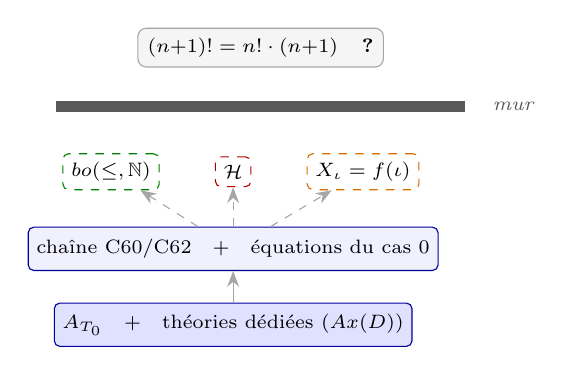
\begin{tikzpicture}[node distance=5mm and 7mm]
\node[goal, draw=gray!70, fill=gray!8] (P) {$(n{+}1)! = n!\cdot(n{+}1)$ \; \textbf{?}};
\node[below=3mm of P, font=\scriptsize\itshape, gray!70!black] (mur)
  {\rule{52mm}{1.4mm}};
\node[right=1mm of mur, font=\scriptsize\itshape, gray!70!black] {mur};
\node[open, draw=green!50!black, below=4mm of mur, xshift=-19mm] (bo)
  {$bo(\le,\mathbb{N})$};
\node[open, draw=red!70!black, right=of bo] (hg) {$\mathcal{H}$};
\node[open, draw=orange!85!black, right=of hg] (hw) {$X_\iota = f(\iota)$};
\node[th, below=5mm of hg] (chain) {chaîne C60/C62 \; + \; équations du cas 0};
\node[ax, below=4mm of chain] (axs)
  {$A_{T_0}$ \; + \; théories dédiées $(Ax(D))$};
\draw[fl] (axs) -- (chain);
\draw[fl, dashed] (chain) -- (bo);
\draw[fl, dashed] (chain) -- (hg);
\draw[fl, dashed] (chain) -- (hw);
\end{tikzpicture}}
\caption{Un mur réel~: la dernière équation ouverte du front factorielle. Les boîtes
pleines sont des objets du noyau, les boîtes en tirets les hypothèses que la chaîne
de dérivation laisse \emph{ouvertes}, et la barre est le mur qui les sépare du but.
La couleur d'une boîte est son verdict de trichotomie, détaillé au
tableau~\ref{tab:frontier}.}
\label{fig:wall}
\end{figure}

\begin{table}[t]\centering\footnotesize
\begin{tabular}{llll}
\toprule
hypothèse ouverte & rencontrée sur & verdict & issue \\
\midrule
$bo(\le,\mathbb{N})$ & la route C62-existence
  & \textcolor{green!50!black}{déchargeable}
  & déclarée irréductible, prouvée close ensuite \\
$\mathcal{H}$ & la route du cas $0$
  & \textcolor{red!70!black}{réfutable}
  & source de la vacuité~; théorème révoqué \\
$H_2$, $H_3$ & le pas de récurrence
  & \textcolor{green!50!black}{déchargeable}
  & tombées avec la réparation de la sec.~\ref{sec:fidelity} \\
$H_W$, $H_N$ & le pas de récurrence
  & \textcolor{orange!85!black}{indépendantes}
  & aucune recherche ne les ferme~; seule la théorie change \\
\bottomrule
\end{tabular}
\caption{La frontière du front, agrégée sur ses routes plutôt que prise sur un
instantané unique du journal. Le résidu mesuré du pas de récurrence était
$\{n{\in}\mathbb{N}, H_2, H_3, H_W, H_N\}$, et la trichotomie l'a scindé. Chaque
ligne est un cas mesuré, et chaque échec est enregistré comme objet certifié.}
\label{tab:frontier}
\end{table}

\begin{table}[h]\centering\footnotesize
\setlength{\tabcolsep}{4.5pt}
\begin{tabular}{lllp{4.3cm}}
\toprule
classe & définition & certificat valide & cas mesuré \\
\midrule
E1 dérive & $C \neq C^\ast$ & comparaison syntaxique & $\mathit{membre\_but}$ (6\,908 $\to$ 8\,592 car.) \\
E2 vacuité & $\{h\} \vdash \bot$ & théorème de conclusion $\bot$ & $\mathcal{H}$ / $0! = 1$ révoqué \\
E3 impasse & aucune continuation ne clôt & élague les extensions & la route « $n{-}1$ » (terme de différence opaque), év.~84--85 \\
E4 dette & $Ax(D) \not\subseteq \{T_0\}{\times}A_{T_0}$ & mesure en process frais & $n\_bien\_ordonne$~: 53 axiomes étrangers \\
E5 fantôme & résidu déjà prouvable & théorème clos $=$ résidu & $bo(\le,\mathbb{N})$, 9 cas au total \\
E6 infidélité & $A_{T_0} \cup \Phi \vdash \bot$ & dérivation close $+$ ancre source & deux défauts d'axiome (sec.~\ref{sec:fidelity}) \\
E7 mesure & la sonde a menti & contre-mesure & sonde à noms devinés (faux négatif) \\
\bottomrule
\end{tabular}
\caption{La taxonomie des échecs \emph{telle que nous l'avons identifiée}. Chaque classe
listée est instanciée par un cas réel de la semaine instrumentée, vérifié par le noyau.
La liste est \textbf{ouverte}~: rien ici ne montre que sept soit tout ce qu'il y a.}
\end{table}

\paragraph{La taxonomie est ouverte, et ne se referme pas par les mêmes moyens que le
reste.} Nous écrivons $\mathcal{K}$ pour l'ensemble des classes d'échec et
$|\mathcal{K}| \ge 7$ plutôt que $\kappa \in \{E1,\dots,E7\}$, parce que la seconde
notation affirme ce que nous n'avons pas établi. Sept classes ont été identifiées et
chacune instanciée par un cas réel~; qu'il existe un échec n'entrant dans aucune n'est ni
exclu ni exclusible ici. Les classes ont été trouvées en regardant des échecs, non
dérivées d'un principe~: le catalogue s'accroît donc par rencontre, et un échec ne
correspondant à aucun $\kappa$ devient $E8$.

L'asymétrie est celle que cet article rencontre deux fois ailleurs. L'infidélité est
semi-décidable --- on peut toujours en \emph{trouver} une, jamais certifier leur absence
(section~\ref{sec:fidelity})~; la nouveauté de même (section~\ref{sec:related}).
L'exhaustivité de $\mathcal{K}$ est de cette famille~: exhiber une huitième classe est un
acte fini, prouver qu'il n'y en a pas ne l'est pas. Nous rapportons donc un catalogue
avec une borne inférieure, non un type à sept habitants --- et nous préférons qu'un
lecteur trouve un $E8$ plutôt qu'il croie la liste close parce que nous l'avons composée
entre accolades.

%% ============================================================================
\section{Fidélité mécanisée~: quand le corpus réfute le livre}
%% ANCRE: CAMPAGNE_DEMOS (26-27 juil + 1 aout) ; derivation D1 ; @livre 2181 notions
%% ============================================================================
\label{sec:fidelity}
\subsection{La discipline d'ancrage et le verdict d'infidélité}
Chaque notion formalisée porte un ancrage lisible par la machine
\texttt{@livre Ch.X \S{}s.ss Type.n | E X.pp L.a-b | PDF p.n} qui la relie à la source
imprimée (2\,234 notions ancrées à l'heure où nous écrivons). L'ancrage a deux champs de
fiabilité inégale, et nous les séparons parce que nous les avons mesurés.

\paragraph{La page est sûre~; l'intervalle de lignes ne l'est pas uniformément.} C'est le
champ « page » qui porte les résultats de couverture ci-dessous~: zéro ancrage non
conforme, et cinq parties du livre déclarées complètes sur leur intervalle. L'intervalle
de lignes est plus faible, et nous l'avons découvert en auditant nos propres ancrages
contre le livre. Sur la page E~II.22 --- 36 lignes imprimées, comptées à la main --- la
Définition~1 occupe les lignes 15--18 et la Définition~2 les lignes 27--30, tandis que
leurs ancrages disent \texttt{L.31-36} et \texttt{L.49-53}~; le second dépasse la page.
Or la ligne 53 de notre \emph{transcription} \LaTeX{} de cette page est exactement
l'en-tête de la Définition~2~: ces deux ancrages indexent la transcription, pas le livre.
Sur la page E~II.7, l'inverse --- l'ancrage suit la ligne imprimée à un petit décalage
près et ne correspond pas du tout à la transcription. Au moins deux conventions coexistent
dans le corpus.

Mesuré sur les 1\,992 ancrages portant un intervalle de lignes~: \textbf{12,2\,\%
finissent au-delà de la ligne 36}, soit environ une page pleine de cette édition, et ne
peuvent donc pas être des références à des lignes imprimées~; le maximum est 63. Le gros
de la distribution a la forme d'une page imprimée, avec une queue qui n'en a pas.

Nous revendiquons donc la traçabilité \emph{à la granularité de la page}, qui est ce que
les instruments de couverture consomment réellement, et nous présentons les intervalles
de lignes intra-page comme une \emph{heuristique} de localisation du matériel non
formalisé plutôt que comme une mesure certifiée. C'est une revendication plus faible que
celle que cet article portait en brouillon, et la raison de la consigner ici est que
c'est la thèse même de l'article retournée contre lui~: aucun test d'un dépôt vérifié par
noyau n'attrape un ancrage qui décrit mal le livre, et les nôtres sont restés inexaminés
jusqu'à ce que nous ouvrions les pages. Soit $\Phi$ la transcription des énoncés numérotés du livre. La fidélité
elle-même --- « $\varphi(b)$ \emph{signifie} $b$ », pour un énoncé $b$ du livre et sa
formalisation $\varphi(b)$ --- relie du texte à des formules et
n'est pas formalisable~; sa négation, si~:
\[
\mathit{Infid} \iff A_{T_0} \cup \Phi \vdash \bot .
\]
$\mathit{Infid}$ est semi-décidable~: on peut toujours \emph{trouver} une infidélité,
jamais certifier son absence --- c'est pourquoi notre audit est un processus permanent
plutôt qu'un pourcentage de couverture. Deux conséquences de la discipline sont
mécanisables gratuitement~: deux ancres citant la même phrase à des lignes différentes
exposent une erreur par simple comparaison (deux cas réels trouvés et corrigés)~; et un
numéro de ligne recopié se propage --- une valeur fausse a été trouvée répliquée
verbatim sur cinq sites.

L'autoformalisation récente à l'échelle du projet enregistre elle aussi la provenance
au niveau de l'empan~; l'état de l'art, M2F~\cite{m2f2026}, impose ensuite la fidélité
des énoncés « par un \emph{audit manuel} relié à la provenance » (p.~8). Notre écart
est exactement là~: le verdict d'infidélité est \emph{dérivé}. Les deux défauts
ci-dessous ont été établis en prouvant une contradiction dans le noyau, et les deux
réparations ont été prouvées efficaces par l'impossibilité de la re-dériver.

Un troisième défaut, trouvé la même semaine, a amorcé la méthode. L'axiome
d'intersection avait été transcrit depuis le \emph{Résumé des résultats} du livre
(E~R.19), dont l'univers de familles de \emph{parties} rend $\bigcap_{\emptyset} = E$
légitime, plutôt que depuis E~II.22, dont la Définition~2 exige $I \neq \emptyset$ (et
dont la note de bas de page avertit que l'intersection non restreinte n'est pas
collectivisante). La théorie de référence elle-même était donc
incohérente. Le défaut a été localisé par preuve machine, son périmètre calculé à
34 sites, et réparé en restaurant la forme de sélection, en maintenant le compte
d'axiomes à 22~; l'incident était clos, suite au vert, avant que la moindre mesure de
dette rapportée dans cet article ne soit prise. Les deux cas ci-dessous ont ensuite été
trouvés \emph{par} la discipline que ce premier incident a instituée.

\subsection{Cas 1~: un axiome a perdu un conjoint}
L'axiome de produit d'une famille avait perdu la borne que le livre impose aux graphes
qu'il admet~: pour une famille $(X_\iota)_{\iota \in I}$ d'ensembles indexée par $I$,
un membre $F$ du produit doit vérifier
$F \subset I \times \bigcup_{\iota \in I} X_\iota$ (son frère, l'axiome
d'exponentiation, avait gardé la sienne). Le corpus démontrait alors, à \emph{zéro}
hypothèse et pour toute famille $u$, à la fois
$\{\emptyset\} \in \prod(u,\emptyset)$ et
$\neg(\prod(u,\emptyset) = \{\emptyset\})$ --- alors que E~II.32 énonce que le produit
vide a exactement un élément. Le corpus réfutait le livre. La correction n'a jamais été
en cause~: le noyau dérivait fidèlement depuis l'axiome qu'on lui avait donné~; c'est
l'axiome qui n'était pas celui du livre. La réparation a restauré le conjoint \emph{en
position de tête} (un choix empirique~: 18 tests cassés contre 33 pour la position de
queue), a maintenu le compte d'axiomes à 22 (remplacement, non ajout), et a payé
immédiatement~: deux hypothèses portées pendant des semaines sont devenues des
théorèmes, et le $0! = 1$ vacueux de la section~\ref{sec:certified-failure} a été
réhabilité par décharge.
La figure~\ref{fig:proofgraph} montre cette dérivation réhabilitée, la branche
que le défaut bloquait étant marquée en vert.

\begin{figure}[t]\centering
\resizebox{\ifdim\width>\linewidth \linewidth\else\width\fi}{!}{%
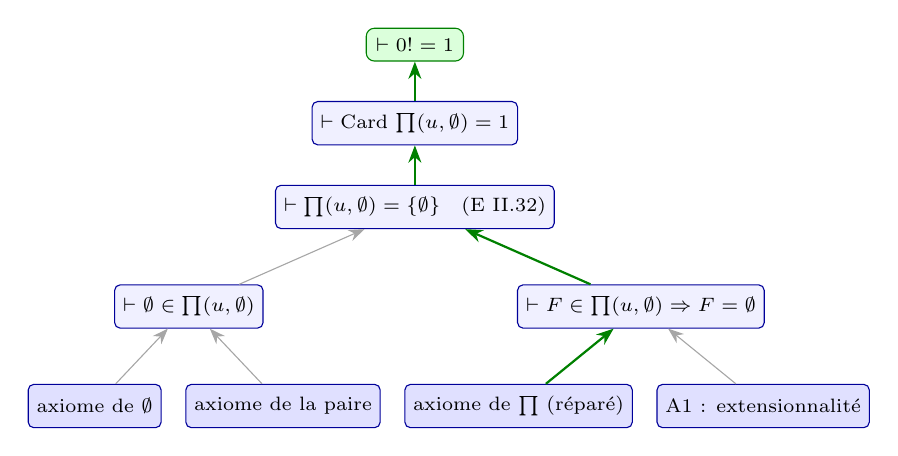
\begin{tikzpicture}[node distance=4mm and 3mm]
\node[ax] (vide) {axiome de $\emptyset$};
\node[ax, right=of vide] (paire) {axiome de la paire};
\node[ax, right=of paire] (prod) {axiome de $\prod$ (réparé)};
\node[ax, right=of prod] (ext) {A1~: extensionnalité};
\node[th, above=7mm of $(vide.north)!0.5!(paire.north)$] (hab) {$\vdash \emptyset \in \prod(u,\emptyset)$};
\node[th, above=7mm of $(prod.north)!0.5!(ext.north)$] (uni) {$\vdash F \in \prod(u,\emptyset) \Rightarrow F = \emptyset$};
\node[th, above=7mm of $(hab.north)!0.5!(uni.north)$] (e232) {$\vdash \prod(u,\emptyset) = \{\emptyset\}$ \; (E~II.32)};
\node[th, above=5mm of e232] (card) {$\vdash \mathrm{Card}\,\prod(u,\emptyset) = 1$};
\node[goal, above=5mm of card] (fact) {$\vdash 0! = 1$};
\draw[fl] (vide) -- (hab); \draw[fl] (paire) -- (hab);
\draw[gl] (prod) -- (uni); \draw[fl] (ext) -- (uni);
\draw[fl] (hab) -- (e232); \draw[gl] (uni) -- (e232);
\draw[gl] (e232) -- (card); \draw[gl] (card) -- (fact);
\end{tikzpicture}}
\caption{La dérivation réelle de $0! = 1$ (route Déf.~2) comme graphe à l'intérieur de
la boîte-théorie. \textbf{Lecture}~: chaque boîte est un objet du noyau --- rangée du
bas, les axiomes consommés~; au-dessus, les théorèmes dérivés~; la boîte à fond vert
est le but. Une flèche de $A$ vers $B$ signifie «~$A$ est une prémisse du pas de noyau
qui dérive $B$~». Les \textbf{flèches vertes épaisses} marquent la branche
\emph{indérivable} tant que l'axiome du produit était privé de son conjoint~; les
\textbf{flèches grises fines}, les pas qui n'ont jamais dépendu du défaut. La
dérivation entière est le dividende de la réparation.}
\label{fig:proofgraph}
\end{figure}

\subsection{Cas 2~: un terme a perdu un paramètre}
Le terme $\mathit{seg}(E,x)$ --- le segment initial déterminé par $x$ --- ne portait
pas sa relation d'ordre~: deux ordres différents produisaient le \emph{même} terme,
chacun avec son propre axiome caractéristique, tous deux acceptés à zéro hypothèse sous
un unique nom de théorie. À partir de deux ordres concrets sur un ensemble à deux
éléments, $\vdash \emptyset \in \emptyset$ se dérive en six pas de noyau. Une passe AST
mécanique a ensuite généralisé la trouvaille~: \textbf{21 constructeurs de termes
perdent au moins un paramètre, 11 d'entre eux l'ordre}, avec une seconde contradiction
dérivée pour les intervalles fermés.

\begin{proposition}[Les gardes ne réparent pas les paramètres perdus]
Ajouter l'hypothèse « $R$ est un ordre sur $E$ » à l'axiome caractéristique laisse la
contradiction dérivable~: deux ordres \emph{différents} sur le même $E$ satisfont tous
deux la garde. Une \emph{condition} perdue peut être restaurée par une garde (cas 1)~;
un \emph{paramètre} perdu, non --- aucune condition ne répare un terme qui n'a pas
d'emplacement pour l'accueillir.
\end{proposition}

Le remède structurel~: le terme porte son graphe --- $\mathit{seg}(G,E,x)$, pour un
graphe $G$, un ensemble $E$ et un point $x$ --- et l'axiome
est $\forall$-clos sur $G$ également. Les quatre instances d'axiome
$\alpha$-distinctes s'effondrent en une seule formule close~; l'usine à théories perd
son paramètre~; et la contradiction devient \emph{structurellement indérivable} --- il
n'existe plus de mécanisme permettant de frapper deux axiomes incompatibles à propos
d'un même terme. Effet de bord~: la clôture supprime la variable libre qui avait permis
au noyau de généraliser sur une \emph{constante} de la théorie ad hoc (une condition de
bord du C27 de Bourbaki que le noyau ne peut pas vérifier, pour la même cause racine
que la dette invisible de la section~\ref{sec:certified-failure}~: les objets théorème
ne portent aucune trace de leur théorie). La suite complète de 3\,909 tests est au vert
sous l'axiome réparé.

\subsection{Le prix de la vérité~: des contradictions porteuses}
La réparation a eu un coût, et le nommer fait partie de la méthode. Deux théorèmes
intermédiaires avaient éliminé le $\exists R_o$ de Zermelo \emph{parce que} le terme de
segment ne portait pas son ordre --- leur prétendue « indépendance en $R_o$ » était un
artefact du défaut. Après réparation, le noyau refuse à juste titre la
généralisation~; les énoncés ont été reformulés sous forme $R_o$-close, et la perte est
nommée~: \emph{Zermelo seul ne suffit plus} pour ces deux réductions --- le bon ordre
et la réalisation des segments par lui doivent être supposés ensemble. Les énoncés plus
forts n'étaient démontrables qu'à travers l'incohérence. C'est le dual mesuré de la
vacuité~: la vacuité est un théorème né mort sous une hypothèse réfutable~; ici un
théorème \emph{meurt avec} le défaut qui le portait. Un audit d'incohérence doit donc
regarder dans les deux sens~: vers ce que le défaut rend faussement réfutable, et vers
ce qu'il rend démontrable-mais-illégitime. La documentation locale avait affirmé
l'indépendance de bonne foi --- c'est la théorie ambiante qui mentait.

%% ============================================================================
\section{La boucle de guidage et la couche vectorielle}
%% ANCRE: VECTORISATION.md ; outils_ia/vecteurs/scan_jumeaux.py (prototype juil. 1,7 s ; re-mesure 4-7 s selon machine) ; sobriete-tokens (economie)
%% ============================================================================
\label{sec:vectors}
\subsection{L'équation de guidage}
Une politique nue propose $\pi(a \mid s)$~; branchée sur le corpus, elle propose
$\pi(a \mid s, M(s))$, où $M(s)$ retrouve les murs dont le prédicat couvre $s$, les
couples de remède dont l'état enregistré ressemble à $s$, et les leçons applicables.
$M(s)$ agit sur la direction de trois façons~: il \emph{interdit} (les murs certifiés
élaguent les coups menant à des routes condamnées), \emph{suggère} (un couple de remède
dit~: dans un état comme celui-ci, ce coup-là a échoué et celui-ci a marché), et
\emph{ordonne} (les prémisses les plus proches du but viennent en premier). La
rétroaction se referme à trois échelles de temps~: par coup, le noyau accepte ou refuse
--- le progrès halluciné n'existe pas~; par route, la frontière $\mathit{Ouv}(D)$ et
les classes de trichotomie de ses hypothèses ouvertes donnent une estimation de valeur
sans apprentissage (une route portant une hypothèse d'allure indépendante est condamnée
quel que soit l'effort)~; par campagne, les problèmes du livre clos et la dette totale.

Les retours sont documentés instance par instance plutôt que moyennés~: un squelette de
preuve révoqué, conservé avec son certificat de vacuité, s'est re-dérivé tel quel une
fois que l'axiome réparé a rendu son hypothèse déchargeable --- une reconstruction
complète évitée~; une route certifiée en impasse (un terme de soustraction opaque) nous
a coûté une fois et jamais plus, l'agent suivant prenant directement la forme
$\mathit{succ}(k)$ recommandée~; neuf murs fantômes ont produit la règle permanente
\emph{re-mesurer avant de croire}, après quoi aucune session n'a été perdue sur un mur
inexistant. Les échecs de la boucle sont journalisés avec la même discipline (un
pronostic de triage faux 21 fois sur 21~; un dépassement de budget qui a produit le
protocole de frugalité du projet), et la réserve de validité est énoncée à la
section~\ref{sec:limitations}~: ce sont des instances tracées, non un effet contrôlé.

\subsection{La couche vectorielle et le détecteur d'axiomes jumeaux}
Les formules sont des arbres étiquetés. En notant $\ell_k(v)$ l'étiquette d'un nœud
$v$ après $k$ tours et $h$ une fonction de hachage, le raffinement de
Weisfeiler-Leman
\[ \ell_{k+1}(v) = h\bigl(\ell_k(v), \{\!\!\{\ell_k(u) : u \text{ fils de } v\}\!\!\}\bigr) \]
haché dans $d{=}512$ compartiments pour $k \le 3$ donne un plongement $\varphi(t)$
d'un terme ou d'une formule $t$, déterministe et sans entraînement, comparé par
similarité cosinus --- calculé en
parcourant l'arbre abrégé, jamais en l'imprimant. Deux leçons de conception ont été
apprises à la dure, et mesurées~: une étiquette qui laisse tomber le nom du symbole
fait s'effondrer des axiomes distincts ($\cos = 1{,}0000$ à tort), et un marcheur
ignorant un attribut fils s'arrête à la profondeur un~; la règle corrective est que
\emph{les cartes de traits se valident sur des paires de similarité connue}, la
discipline du test par mutation appliquée aux représentations. La calibration est livrée
sous forme de tests. La paire incohérente d'axiomes $\mathit{seg}$ mesure $0{,}9810$
--- reconstruite en fixture, le défaut lui-même ayant depuis été réparé, afin que le
détecteur conserve un cas positif contre lequel être testé~; deux axiomes d'une même
famille mesurent $0{,}8758$ et une paire véritablement sans rapport $0{,}5415$, si bien
que $\theta = 0{,}90$ sépare avec marge des deux côtés.

Le détecteur signale alors
\[ \mathit{Twin}(\alpha,\beta) \iff \tau(\alpha) \cap \tau(\beta) \neq \emptyset
   \;\wedge\; \mathit{sim}(\alpha,\beta) \geq \theta_{\mathrm{twin}} , \]
un terme caractérisé commun et des corps similaires, évalué sur les paires déjà
retenues à $\theta = 0{,}90$. Il y a deux seuils et non un~: $\theta$ choisit ce qui
mérite un regard, $\theta_{\mathrm{twin}} = 0{,}95$ tranche. La conjonction compte~:
la similarité la plus haute du balayage --- un $1{,}0000$ plein --- relie deux copies
d'une même formule, une théorie ad hoc portant encore l'axiome que la réparation de
l'intersection avait depuis promu dans $A_{T_0}$. Son définiendum appartient au
vocabulaire propre de $T_0$ et se trouve donc écarté de $\tau$~: aucun terme n'est
partagé, aucune alerte n'est levée --- alors que le score seul aurait déclenché la
plus bruyante du corpus.

Définir $\tau(\alpha)$ a demandé un raffinement de plus, et c'est un faux positif qui
l'a produit. Un premier critère prenait tout symbole propre à un axiome, et appariait
donc l'axiome qui \emph{définit} l'intervalle d'entiers avec un axiome qui se borne à
l'\emph{utiliser} comme borne. Deux axiomes qui mentionnent un terme ne sont pas en
conflit~; seuls deux qui le définissent le sont. Le terme caractérisé est donc le
définiendum --- le membre gauche de l'équivalence définissante --- et rien d'autre. La
distinction n'est pas un détail d'implémentation~: c'est elle qui sépare un score de
similarité d'un verdict, et elle est restée invisible jusqu'à ce que le détecteur
produise une alerte vérifiable à la main.

Le balayage vectorise 65 axiomes de 41 fabriques de théories --- 43 axiomes de
40 théories dédiées, plus les 22 de $T_0$ lui-même, scannés comme témoins --- en
quelques secondes, renvoie 34 paires au-dessus de $\theta$ et \emph{exactement un}
jumeau (deux théories caractérisant un même terme $h\_iso\_max$ à $0{,}9911$, en cours
d'audit)~; 19 usines paramétriques sont sautées et signalées comme telles --- elles sont la classe
à risque elle-même, une usine paramétrique étant précisément le mécanisme qui a rendu
$\mathit{seg}$ incohérent. L'incohérence qui avait coûté une investigation de 95 minutes est
désormais une requête de conformité permanente.

%% ============================================================================
\section{Étude de cas~: une semaine instrumentée}
\label{sec:case-study}
%% ANCRE: CAMPAGNE_DEMOS.md (26 juil - 2 aout) ; events.jsonl (95) ; suites de tests
%% ============================================================================
\label{sec:casestudy}

Nous rapportons une semaine instrumentée (26 juillet -- 2 août 2026) durant laquelle
chaque mécanisme des sections~\ref{sec:certified-failure}--\ref{sec:vectors} a été
exercé sur des mathématiques vivantes --- le chapitre factorielle de la
\emph{Th\'eorie des ensembles} et sa machinerie amont.

\begin{table}[h]\centering\small
\begin{tabular}{lp{7.6cm}}
\toprule
défauts d'axiome trouvés \& réparés & \textbf{3} (un par preuve machine de
l'incohérence de la théorie, deux par contradiction dérivée), tous réparés en
maintenant le compte à 22, guérison prouvée par non-dérivabilité \\
affirmations de la documentation réfutées & ${\sim}\textbf{78}$ le premier jour
d'audit~; un pronostic de triage du directeur mesuré faux \textbf{21/21} par la suite \\
murs fantômes dissous & \textbf{3} cette semaine --- neuf dans le corpus au total ---
des blocages déclarés, mesurés déchargeables ou déjà résolus \\
théorème vacueux & \textbf{1} révoqué (hypothèse réfutable), plus tard
\emph{réhabilité tel quel} par décharge \\
énoncés affaiblis & \textbf{2}, démontrables seulement à travers l'incohérence~; perte
nommée (dual de la vacuité, sec.~\ref{sec:fidelity}) \\
dette invisible mesurée & 4 capstones~: \textbf{53 / 57 / 9 / 82} instances d'axiomes
étrangers derrière des comptes d'hypothèses déclarés de 0 / 10 / 4 / 7 \\
constructeurs perdant des paramètres & \textbf{21} signalés par une seule passe AST~;
11 perdent l'ordre~; 2 contradictions dérivées \\
suite de tests & $3\,850 \to 3\,909$ collectés~; trois passages complets au vert sous
réparations successives, final \textbf{3\,909 / 3\,909} \\
journal d'événements certifiés & \textbf{95} entrées à la fin de la semaine (37
antérieures à la semaine), chacune re-parsée et, le cas échéant, vérifiée par le
noyau \\
économie du détecteur & investigation $\approx 95$ min $\to$ requête quelques s \\
\bottomrule
\end{tabular}
\caption{La semaine instrumentée en chiffres. Chaque chiffre remonte à un événement
journalisé et daté~; les totaux de tests ont augmenté au fil des trois passages au vert
enregistrés --- aucune suite n'a été mise en sourdine pour obtenir le vert.}
\end{table}

Trois épisodes portent l'argument. \emph{(i) Le cycle de réparation complet, deux
fois.} Les deux défauts d'axiome ont parcouru la boucle entière --- détecter par
dérivation, localiser par périmètre mesuré, réparer structurellement, prouver la
contradiction indérivable, re-passer la suite entière ---, démontrant qu'une théorie
ambiante incohérente est un événement mesurable et réparable plutôt qu'une catastrophe.
\emph{(ii) Révocation et réhabilitation.} Le $0! = 1$ vacueux a été révoqué avec son
certificat conservé~; la réparation a transformé son hypothèse réfutable en théorème~;
le squelette identique s'est alors fermé sans résidu et a survécu à une passe
adversariale (quatorze mutants authentiques tués, aucun par exception). Les objets
d'échec ne sont pas des pertes sèches~; ce sont des actifs différés. \emph{(iii) Le
prix de la vérité.} La même réparation a affaibli deux énoncés acquis qui s'appuyaient
sur le défaut --- mesuré, nommé et conservé comme la meilleure preuve que la
contradiction était vivante.

Opérationnellement, la semaine a aussi mesuré sa propre enveloppe~: la photo de
référence de la suite complète a tourné en 2\,h\,43 d'horloge à quatre workers~; les
longues exécutions sont tuées par l'environnement aux alentours de la barre des
50 minutes, si bien que les suites sont découpées en sept zones avec persistance
incrémentale des résultats~; et un dépassement précoce du budget d'agents a produit le
protocole de frugalité sous lequel le balayage de l'état de l'art de la
section~\ref{sec:related} a plus tard renvoyé 69 références triées pour 237k tokens là
où le premier fan-out de la semaine en avait brûlé 266k pour zéro résultat. Le harnais,
lui aussi, fait partie de l'expérience.

\paragraph{Reproductibilité.} Les comptes de tests cités dans l'étude de cas ci-dessus sont ceux de la semaine instrumentée et sont laissés tels que mesurés alors~; pour mémoire, la suite relancée intégralement le 20~août 2026 rend 	extbf{4\,221 passed en 2\,h\,03} à douze workers avec 	exttt{--dist loadfile}. Nous rapportons les deux plutôt que de rétrofitter le récit avec un nombre postérieur.

Toutes les mesures ont été prises sur une seule machine
Windows~11~: Python~3.13, pytest~9.0.3 avec \texttt{pytest-xdist},
\texttt{PYTHONIOENCODING=utf-8}, suites découpées par zone. L'instrument de dette n'est
valide qu'à la première mesure d'un process frais
(section~\ref{sec:certified-failure})~; le balayage des jumeaux a tourné avec $K = 3$,
$d = 512$, $\theta = 0{,}90$, $\theta_{\mathrm{twin}} = 0{,}95$, et se reproduit par
\texttt{python outils\_ia/vecteurs/scan\_jumeaux.py} --- son plongement hache avec
\texttt{blake2b} plutôt qu'avec le \texttt{hash} de Python, dont la randomisation par
process rendrait irreproductible chacun des cosinus rapportés ici. Le corpus, le
journal et chaque script cité ici sont livrés dans l'instantané du dépôt référencé
en page de titre.

\subsection{Seconde étude de cas~: un énoncé ouvert sous instrumentation}
\label{sec:goldbach}

Deux jours après la semaine rapportée ci-dessus (5--6 août), la même instrumentation a
été tournée vers un énoncé \emph{ouvert}~: la conjecture de Goldbach, écrite sur
l'arithmétique construite du corpus. Nous n'en rapportons ici que ce qui porte sur les
thèses de cet article --- que les défauts d'énoncé se \emph{démontrent} et que la dette
se \emph{mesure}. Les réductions produites par l'épisode, et la mesure de la quantité
d'arithmétique qu'elles contiennent, font l'objet d'un article compagnon~; les organes
de découverte qu'il a exercés relèvent d'un troisième.

\emph{(i) Deux défauts d'énoncé, démontrés dans le noyau.} La première rédaction de la
conjecture disait «~$n$ pair et $n \neq 2$~». Son antécédent est satisfait en $n = 0$ ---
démontré, clos~: $\vdash \mathrm{pair}(0)$ (témoin $k := 0$) et $\vdash \neg(0 = 2)$ ---
de sorte que l'énoncé affirmait que \emph{zéro est somme de deux nombres premiers}.
Réparé, il restait faux~: «~pair~» contraint $n$ à être un \emph{cardinal}, non un
entier, et l'antécédent est aussi satisfait par $n := \mathbb{N} + \mathbb{N}$, qui est
infini --- démontré de même, l'égalité avec l'ancien antécédent instancié étant
vérifiée formule contre formule. La même faute --- un quantificateur portant sur des
ensembles alors qu'on le croit porter sur des entiers --- avait été commise la veille sur
le $(\forall d)$ de la primalité~: c'est un \emph{motif}, désormais consigné.

Fait notable~: la variante bornée \emph{démontrée} de l'énoncé portait la garde de
finitude dès son premier jet, parce que sa preuve l'exigeait~; seul l'énoncé \emph{non
démontré} avait dérivé. \textbf{Démontrer force à nommer ses hypothèses~; énoncer ne
force à rien.} Nous tenons cela pour l'observation la plus transférable de l'épisode, et
c'est pourquoi l'audit de fidélité de la section~\ref{sec:fidelity} vise les énoncés
qu'aucune preuve n'exerce actuellement.

\emph{(ii) La dette, en trois nombres.} «~Zéro hypothèse résiduelle~» et «~l'invariant
des 22 axiomes tient~» se lisent ensemble comme «~ne dépend que des 22~» --- faux au sens
mesuré, puisque les axiomes entrent par la règle d'$\mathrm{axiome}$ et disparaissent du
séquent (section~\ref{sec:certified-failure}). Mesuré en process frais sur la forme
bornée en $n$~: \textbf{0} hypothèse résiduelle~; \textbf{14} des 22 axiomes de
référence consommés~; \textbf{53} formules étrangères --- une seule règle, le critère C54
(le graphe d'une fonction définie par un terme, théorème chez Bourbaki, axiome de
théorie dédiée ici), instanciée 52 fois, plus une instance de Knaster--Tarski. Un
résultat honnête s'annonce avec les trois nombres~; le troisième dit ce qui reste à
dériver.

Sur l'équivalence principale de l'épisode, la même mesure rend \textbf{0}~;
\textbf{14}~; \textbf{73} --- répartis sur \emph{21} théories dédiées, la machinerie du
bon ordre (Zorn, Zermelo, Bourbaki--Witt) entrant par le lemme «~un minorant d'un fini
est fini~». Lever une borne se paie en bon ordre~: le saut de 2 à 21 théories
\emph{mesure} ce que coûte la généralité. La première mesure avait rendu zéro en une
seconde --- le théorème sortait d'un cache, et l'instrument est aveugle à ce qui n'est
pas construit~: la règle du process frais, écrite pour d'autres mesures, s'applique à
elle-même.

\emph{Ce qui est différé.} L'épisode a duré quatre jours et laissé le compte d'axiomes à
22. Sa production mathématique --- une chaîne de réductions certifiées faisant converger
la conjecture sur un seul objet, et la mesure, par paramétrisation du prédicat de
primalité, que ces réductions ne contiennent aucune arithmétique --- est rapportée
séparément, de même que le travail des organes de découverte qu'il a exercés. Rien de
tout cela n'approche la conjecture. Ce qui a sa place ici est la paire de résultats
ci-dessus~: un énoncé ouvert est un endroit particulièrement propice pour attraper un
défaut de fidélité, précisément parce que rien ne le démontre.

%% ============================================================================
\section{Travaux connexes}
%% ANCRE: sources/INDEX.md (16 refs) ; passe systematique OBLIGATOIRE avant soumission
%% ============================================================================
\label{sec:related}
Cette section condense un balayage systématique et adversarial (quatre pistes de
recherche indépendantes, 57 requêtes, 69 références triées, les cinq menaces les plus
proches lues intégralement)~; la méthode du balayage et ses tableaux complets sont dans
le dépôt.

\paragraph{Les systèmes les plus proches.}
Goedel-Architect~\cite{goedelarchitect2026} est le voisin le plus immédiat~: des
graphes de plan dont les n\oe uds en échec portent l'un de \emph{deux} diagnostics ---
énoncé-faux, appuyé par un contre-exemple vérifié par compilateur, ou
preuve-trop-dure, close par un « forfait » structuré. Nos écarts sont au nombre de
trois~: leurs forfaits enregistrent où le prouveur \emph{croit} que se trouve la
lacune (prose non vérifiée) là où nos certificats sont des objets du noyau à périmètre
calculé~; leur boucle vit à l'échelle d'une exécution là où notre corpus persiste et
où les retours sont tracés instance par instance~; et leur diagnostic est binaire là où
notre trichotomie a une troisième branche. AutoformBot~\cite{atlas2026}, le système
derrière la bibliothèque ATLAS, publie la \emph{forme} de la boucle --- des analyseurs
de traces persistants maintiennent des « skill guides » que les workers doivent lire
avant de réessayer --- et un critère de succès délibérément non transitif~; nos
revendications ne reposent donc pas sur la boucle mais sur la certification de ses
maillons et sur la dette par dérivation. Les agents prouveurs
auto-modifiants~\cite{selfmodifying2026} co-évoluent avec un score de benchmark plutôt
qu'avec un journal certifié.

\paragraph{Données d'échec et réparation de preuves.}
REPLica~\cite{ringer2020replica} a capturé des tentatives humaines ratées et des
couples annulation-réparation à état constant --- le format qu'adoptent nos événements
de remède. La lignée de la vérification de programmes transforme les preuves ratées en
artefacts structurés~: un test exécutable dérivé d'un
contre-exemple~\cite{huang2023proof2test} avec une taxonomie de diagnostic à trois
causes~\cite{petiot2016fails}. La réparation est désormais une industrie~: par
transformation~\cite{ringer2018pumpkin}, à l'échelle d'un
jeu de données~\cite{reichel2023proofrepair},
conditionnée par le message d'erreur~\cite{first2023baldur,april2026},
locale au plan~\cite{blueprintrepair2026}.
Il existe des taxonomies d'erreurs pour les tentatives humaines~\cite{aitken2000errors},
les incompatibilités de version~\cite{hou2025versions} et les défauts de
benchmark~\cite{faults2026} --- ce dernier étant le seul autre travail que nous ayons
trouvé qui \emph{certifie} les défauts qu'il rapporte. Aucun de ceux-ci ne certifie un
échec de recherche dans le noyau, ne calcule son périmètre d'invalidation, ni ne le
conserve lorsque aucune réparation n'existe.

\paragraph{Fidélité et Bourbaki.}
La provenance au niveau de l'empan vers les textes sources est désormais standard à
l'échelle d'un projet~\cite{m2f2026,proofnet2023}, et la certification de fidélité est
un sujet actif en 2026~\cite{faithfulnessgap2026,formalrx2026}~; la différence
décisive, argumentée à la section~\ref{sec:fidelity}, est que le verdict de l'état de
l'art est estimé ou manuel là où le nôtre est dérivé. L'audit de
preuves~\cite{adams2016auditing} et la détection d'incohérences dans de grandes bases
du premier ordre~\cite{schulz2017inconsistencies} poursuivent la correction d'une base
pour elle-même, sans texte source ni guérison certifiée. Sur le formalisme~:
Gaia~\cite{grimm2010gaia} formalise le \emph{contenu} de Bourbaki au-dessus de Coq et
laisse le chapitre~I décrit mais inhabité~; la pathologie de taille est
classique~\cite{mathias2002term}~; des noyaux LCF modernes existent en
Python~\cite{knuckledragger} et au-dessus de la théorie des ensembles
standard~\cite{guilloud2023lisa}, si bien que le véhicule n'est pas la nouveauté ---
c'est le formalisme habité qui l'est.

\paragraph{Réparation, révision et formation de théories.}
La réparation automatisée de théories est un programme
établi~\cite{li2022abc,li2022entrenchment,troquard2018weakening}, fondé sur la révision
AGM~\cite{agm1985}~; ses diagnostics sont heuristiques et ses remèdes validés
empiriquement, non par un changement de dérivabilité dans un noyau. Un Lakatos
computationnel existe~\cite{pease2007lakatos} et l'exploration de théories découvre de
vrais lemmes~\cite{johansson2014hipster}~; les deux jettent leurs échecs. La réfutation
est industrialisée, de Nitpick~\cite{blanchette2011nitpick} à la génération de
contre-exemples à l'échelle des LLM~\cite{learningtodisprove2026} --- la branche
réfutable de notre trichotomie~; nous avons mesuré que cette dernière ne mentionne
jamais un troisième statut, et l'enquête de référence 2026 du
domaine~\cite{conjecturingsurvey2026} organise le champ selon des axes orthogonaux au
statut logique.

\paragraph{Guidage, plongements, environnements, mémoire.}
Les traits structurels de formules pour les grandes théories ont une
décennie~\cite{kaliszyk2015features}, avec des plongements appris invariants par
symbole~\cite{olsak2020invariant,jakubuv2020enigma} guidant la saturation et la
sélection de prémisses~\cite{alemi2016deepmath,mikula2023magnushammer}~; notre
détecteur partage l'objectif d'invariance mais est sans entraînement (WL
exact~\cite{shervashidze2011wl}) et résout un problème différent --- la coïncidence
inter-théories d'axiomes caractéristiques, une tâche que nous avons trouvée non
traitée. Le noyau-comme-environnement est
mature~\cite{yang2019coqgym,lample2022htps,polu2020gptf}~; les mémoires de compétences
d'agents validées par exécution~\cite{wang2023voyager} et l'apprentissage de
bibliothèques en veille-sommeil~\cite{ellis2021dreamcoder} sont les ancêtres de la
boucle hors des mathématiques. La structure de dépendances des bibliothèques est
analysée à grande échelle~\cite{mathlibnetwork2026,atlas2026}, topologiquement~; nous
n'avons trouvé aucune métrique nommée de dette d'axiomes par dérivation. Le cadre de
déploiement lui-même --- l'ingénierie déployée chez le client et l'ingénierie de
contexte / de harnais --- vient d'acquérir une taxonomie et des critères de
qualité~\cite{fde2026taxonomy,contextengineering2026}~; cet article peut se lire comme
une instance instrumentée et adossée à un vérificateur de cette pratique.

\paragraph{La nouveauté, énoncée honnêtement.}
Les revendications de nouveauté sont semi-décidables~: on peut prouver la non-nouveauté
en exhibant l'article, jamais la nouveauté. Notre revendication est donc
méthodologique~: après un balayage adversarial documenté, aucun contre-exemple n'a été
trouvé à aucun des points suivants --- des objets d'échec certifiés par le noyau à
périmètre calculé~; une troisième branche (indépendance) opérationnelle~; un verdict
d'infidélité mécanisé et fondé sur une dérivation contre une source imprimée
préexistante~; une mesure nommée de dette d'axiomes par dérivation~; une détection
d'axiomes jumeaux sans entraînement~; un chapitre~I habité.

%% ============================================================================
\section{Limites et menaces sur la validité}
%% ============================================================================
\label{sec:limitations}
\paragraph{Un seul esprit.} Le système a été conçu, exploité et audité par un unique
auteur-opérateur (avec des agents LLM sous sa direction). Les passes de vérification
adversariale sont institutionnalisées précisément parce que le directeur n'est pas
digne de confiance~: un pronostic de triage a plus tard été mesuré faux sur ses
21 prédictions, et cet épisode est journalisé avec la même discipline que les succès.
Reste que la réplication indépendante est le vrai test, et le corpus est publié pour la
rendre possible.

\paragraph{Des retours observationnels.} Les retours de la boucle de guidage
(section~\ref{sec:vectors}) sont des instances tracées, non un effet contrôlé~: la
semaine ne peut pas être rejouée sans son corpus pour mesurer un contrefactuel. Ce qui
survit à cette réserve~: chaque instance est datée et journalisée aux deux bouts
(l'échec et la réutilisation), plusieurs gains sont des rapports mécaniques
indépendants de tout contrefactuel (95 minutes contre quelques secondes~; un blocage déclaré
sur plusieurs sessions mesuré résolu en 4,7 secondes), et les échecs de la boucle sont
enregistrés avec une discipline égale.

\paragraph{Échelle.} 232 événements certifiés, 8 mesures de dette,
60 fabriques de théories dédiées,
un livre. Chaque revendication de cet article est une revendication d'existence ou
d'instance, jamais une revendication statistique. L'instrument de dette n'est valide
qu'au premier appel d'un process frais (sous-comptage mesuré de $-62\,\%$ sinon)~; la
suite complète tourne en 2\,h\,03 à douze workers (2\,h\,43 aux quatre de la semaine rapportée ici) et l'environnement tue les longues
exécutions vers 50 minutes, ce qui borne le délai expérimental et a dicté la discipline
de découpage.

\paragraph{Zones connues non mesurées.} La qualité des assertions des tests hors des
fichiers que nous avons édités (une dérive pourrait se cacher ailleurs derrière un test
ne vérifiant que la clôture)~; les 19 usines paramétriques de théories que le détecteur
de jumeaux ne couvre pas encore --- la classe à risque elle-même~; la suffisance en
aval des deux énoncés délibérément affaiblis~; la condition de bord de C27 dans le
noyau, documentée comme dette de conception et laissée intacte par règle de projet~;
un écart de fidélité nommé ($\sup$ contre maximum dans le $M(u)$ de C63) assumé et
confiné. La nouveauté repose sur un balayage adversarial documenté et est
semi-décidable par nature~; les cinq menaces les plus proches ont été vérifiées contre
leurs PDF complets, et chaque liste d'auteurs restante contre sa page arXiv ou
d'éditeur.

\paragraph{Généralisabilité.} Tout ce qui précède jouit d'un oracle exact. Le transfert
du cadre à des domaines à oracle bruité --- où les certificats deviennent statistiques
--- est plausible mais non testé~; nous revendiquons la limite à bruit nul, non le cas
général.

%% ============================================================================
\section{Conclusion~: vers une IA qui crée des théories}
%% ANCRE: annexe justification substrat (R1-R10) ; VECTORISATION 3-6
%% ============================================================================
Le but que sert ce substrat est une IA qui \emph{crée des théories} pour résoudre des
problèmes. Dériver les exigences de ce but --- des théories comme données de première
classe et bon marché~; un vérificateur exact et infalsifiable~; une dette traçable~;
des objets inventés comme termes~; un corpus de \emph{processus}, échecs compris~; une
métathéorie disponible à l'intérieur du système~; une réserve de couples $(T,P)$ avec
un gradient de difficulté~; des coups locaux composables~; une identité à travers les
révisions~; le transport entre théories --- donne une liste que nous gardons
explicitement \emph{ouverte}~: elle a elle-même été prouvée incomplète une fois, par
les mêmes chasses adversariales qui auditent tout le reste ici, et la complétude d'une
telle liste est exactement aussi semi-décidable que la fidélité. Le système décrit dans
cet article en satisfait le c\oe ur, et la semaine instrumentée est la preuve
d'existence que la partie difficile --- le cycle complet \emph{détecter par dérivation,
localiser par périmètre mesuré, réparer structurellement, prouver la guérison, nommer
le coût} --- tourne de bout en bout sur des mathématiques vivantes, deux fois.

\begin{figure}[t]\centering
\resizebox{\ifdim\width>\linewidth \linewidth\else\width\fi}{!}{%
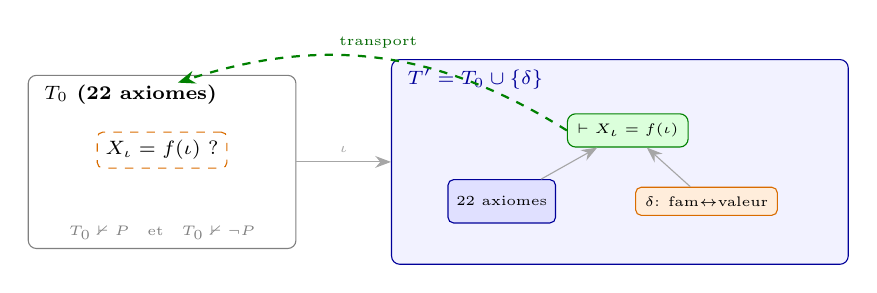
\begin{tikzpicture}[node distance=5mm and 8mm]
\node[draw=gray, rounded corners=3pt, minimum width=34mm, minimum height=22mm, font=\scriptsize] (T0) {};
\node[font=\scriptsize\bfseries, anchor=north west] at (T0.north west) {\;$T_0$ (22 axiomes)};
\node[open, draw=orange!85!black, font=\scriptsize] at ($(T0.center)+(0,1.5mm)$) {$X_\iota = f(\iota)$ ?};
\node[font=\tiny, gray, anchor=south] at (T0.south) {$T_0 \nvdash P$ \; et \; $T_0 \nvdash \neg P$};
\node[draw=blue!60!black, fill=blue!5, rounded corners=3pt, minimum width=58mm, minimum height=26mm, right=12mm of T0, font=\scriptsize] (T1) {};
\node[font=\scriptsize\bfseries, anchor=north west, blue!60!black] at (T1.north west) {\;$T' = T_0 \cup \{\delta\}$};
\node[ax, font=\tiny] at ($(T1.center)+(-15mm,-5mm)$) (a22) {22 axiomes};
\node[draw=orange!85!black, fill=orange!14, rounded corners=2pt, font=\tiny] at ($(T1.center)+(11mm,-5mm)$) (delta) {$\delta$: fam$\leftrightarrow$valeur};
\node[goal, font=\tiny] at ($(T1.center)+(1mm,4mm)$) (iP) {$\vdash X_\iota = f(\iota)$};
\draw[fl] (a22) -- (iP); \draw[fl] (delta) -- (iP);
\draw[fl] (T0.east) -- node[above, font=\tiny] {$\iota$} (T1.west);
\draw[gl, dashed] (iP.west) to[bend right=25] node[above, font=\tiny, green!40!black] {transport} ($(T0.north)+(2mm,-1mm)$);
\end{tikzpicture}}
\caption{Le coup que seul un substrat où la théorie est une donnée permet.
\textbf{Lecture}~: chaque grand rectangle arrondi est une \emph{théorie} (à gauche la
référence $T_0$, à droite son extension $T'$)~; à l'intérieur, les boîtes bleues sont
des axiomes, la boîte \textbf{orange} la définition $\delta$ ajoutée (et, à gauche,
l'hypothèse orange à laquelle elle répond), la boîte verte le but désormais
démontrable~; la \textbf{flèche verte en tirets} est le transport du résultat en
retour dans le langage de $T_0$. Quand une
hypothèse est \emph{indépendante} (ici le pont famille-valeur, indépendant de
$A_{T_0}$), aucune recherche ne la ferme --- le seul coup légal étend la théorie par
une définition $\delta$, démontre l'image, et transporte le résultat en retour.}
\label{fig:extension}
\end{figure}

Lu abstraitement, le système est une enquête expérimentale dans la limite à bruit
nul~: la falsification est une dérivation, la révision de théorie est une opération
exécutable au résultat certifié, la sévérité d'un test est un compte de mutants, et
l'économie de la mesure est un budget aux dépassements journalisés --- Popper, Lakatos,
Mayo et AGM comme code qui tourne plutôt que comme philosophie des sciences. C'est
cette limite qui rend le corpus précieux comme données d'entraînement~: chaque
étiquette est exacte.

La feuille de route découle des mesures. Une instrumentation de rejeu transforme le
corpus existant de 4\,221 tests en $10^5$--$10^6$ tuples certifiés (état, action,
verdict) sans formaliser une seule page nouvelle --- l'usine à données est la même
infrastructure que le cache de termes qui supprime le coût dominant de reconstruction.
Une API d'environnement ($\mathit{reset}(T,P)$ / $\mathit{step}$) expose la boucle à
n'importe quelle politique~: les modèles de pointe sont loués et remplaçables~; ce sont
la mémoire de guidage $M(s)$ et ses étiquettes certifiées qui s'accumulent et
qu'aucun corpus de preuves existant ne fournit. La seconde version du détecteur de
jumeaux lit le terme caractérisé dans la forme de l'axiome et couvre les usines
paramétriques. Et la frontière stratégique est le chapitre~IV de Bourbaki ---
structures et transport --- parce que c'est là qu'une théorie créée pour un problème
apprend à rapporter dans un autre.

Un assistant de preuve certifie ce que nous savons. Un corpus d'échecs certifiés
enregistre comment nous en sommes venus à le savoir --- les murs, les réparations, les
prix payés --- et pour une machine qui doit apprendre à \emph{créer} des théories
plutôt qu'à chercher à l'intérieur d'une seule, c'est la denrée la plus rare.

\bibliographystyle{plain}
\bibliography{references}

\end{document}
